\title{The Temporal-Sparsity Dilemma: Challenges in Learning Time-Aware Features from Language Model Activations}

% Comment: Title section introduces the novel approach of incorporating temporal information into SAEs
\author{Anonymous Authors}
\date{\today}

\begin{document}
\maketitle

% Comment: Abstract paragraph structure:
% 1. Context and motivation
% 2. Current limitations and challenges
% 3. Our proposed solution
% 4. Methods and implementation
% 5. Results and implications
\begin{abstract}
Understanding how large language models (LLMs) process sequential information remains a fundamental challenge in AI interpretability. While Sparse Autoencoders (SAEs) have emerged as powerful tools for analyzing neural activations, they currently ignore the temporal relationships inherent in language processing by treating each activation independently. We present Temporal Sparse Autoencoders (TSAEs), which extend traditional SAEs with position-aware embeddings and temporal coherence constraints to capture sequential dependencies in LLM representations. However, our systematic experiments on the Gemma-2B model reveal fundamental tensions between temporal coherence and sparse feature extraction. Despite implementing extensive stability measures including gradient clipping, batch normalization, and conservative learning rates (5e-5), all architectural variants exhibited complete feature collapse ($l_0$ and $l_1$ sparsity at 0.0) with poor reconstruction quality (MSE 47.25). These results, supported by detailed ablation studies across layers 5, 12, and 19, demonstrate critical challenges in combining temporal awareness with sparse feature learning, suggesting the need for fundamentally new approaches to temporal-aware neural interpretation.
\end{abstract}

\section{Introduction}
Understanding how large language models (LLMs) process sequential information remains a fundamental challenge in AI interpretability. While Sparse Autoencoders (SAEs) have emerged as powerful tools for analyzing neural activations \cite{anthropic2022decomposition}, they currently ignore the temporal relationships inherent in language processing by treating each activation independently. This limitation is particularly critical as sequential dependencies are fundamental to how LLMs process and generate text.

The challenge lies in combining two competing objectives: learning sparse, interpretable features while preserving temporal coherence. Traditional SAEs achieve sparsity through $l_1$ regularization and learned dictionaries, but enforcing temporal consistency introduces complex optimization dynamics that can destabilize training. Previous attempts to incorporate temporal information in neural interpretability have focused on causal tracing \cite{elhage2022solu} rather than feature learning.

We present Temporal Sparse Autoencoders (TSAEs), which extend traditional SAEs with position-aware embeddings and temporal coherence constraints. Our key innovations include:
\begin{itemize}
    \item A novel architecture combining learned position embeddings (dimension=32) with adaptive feature thresholding
    \item A temporal coherence loss (weight=0.01) that encourages consistency across sequential positions
    \item Comprehensive stability measures including gradient clipping, batch normalization, and conservative learning rates
\end{itemize}

Through systematic experimentation on the Gemma-2B model across layers 5, 12, and 19, we reveal fundamental tensions between temporal coherence and sparse feature extraction. Despite implementing extensive stability measures, all architectural variants exhibited complete feature collapse ($l_0$ and $l_1$ sparsity at 0.0) with poor reconstruction quality (MSE 47.25). Our results, supported by detailed ablation studies shown in Figure~\ref{fig:training_metrics}, demonstrate that these challenges persist even with simplified architectures and conservative optimization strategies.

The consistent training failures across five distinct architectural variants, documented in Figure~\ref{fig:architecture_comparison}, suggest deeper theoretical tensions between temporal coherence and sparse representation learning. These findings advance our understanding of temporal-aware interpretation methods and highlight critical challenges that must be addressed to develop effective tools for analyzing sequential processing in LLMs.

% Comment: Structure of Related Work section
% 1. Prior work on interpreting temporal aspects of LLMs
% - Compare with \cite{elhage2022solu}'s approach to analyzing sequential information flow
% - Contrast with traditional activation analysis methods that ignore temporal dependencies
%
% 2. Sparse representation learning in neural networks
% - Build on \cite{anthropic2022decomposition}'s SAE framework
% - Discuss key differences in handling temporal coherence vs static sparsity
%
% 3. Temporal coherence in representation learning
% - Relate to work on temporal consistency in other domains, where approaches like life-time sparsity have been shown to effectively capture temporal coherence in feature learning \cite{Springenberg2012LearningTC,Sahu2020CrossmodalNG},
% - Highlight unique challenges in LLM context
%
% 4. Optimization challenges in sparse-temporal learning
% - Connect to broader literature on training stability
% - Emphasize novel aspects of our stability issues

\section{Related Work}
Three main research directions inform our work: temporal analysis of language models, sparse feature learning, and optimization challenges in deep networks. \cite{elhage2022solu} pioneered the analysis of temporal dependencies in transformers through causal tracing, revealing how information flows across attention layers. While their method effectively tracks existing temporal patterns, it cannot learn new interpretable features - a key goal of our work. Their findings about information flow stability influenced our position embedding design, though our results (MSE 47.25) suggest additional challenges in learning stable temporal features.

The sparse autoencoder framework of \cite{anthropic2022decomposition} forms our methodological foundation. Their approach successfully learns interpretable features from static activations using L1 regularization and learned dictionaries. However, they explicitly avoid temporal dependencies by treating each position independently. Our work reveals fundamental tensions when attempting to combine their sparsity constraints with temporal coherence - all variants exhibited complete feature collapse ($l_0$ and $l_1$ sparsity at 0.0) despite using their proven optimization techniques.

The training instabilities we encountered connect to broader optimization challenges studied by \cite{Glorot2010UnderstandingTD}. While they identified gradient flow issues in deep networks, our problems persist even with modern solutions like batch normalization and gradient clipping. As shown in Figure~\ref{fig:training_metrics}, conservative learning rates (5e-5) and large batches (4096) failed to prevent collapse, suggesting unique difficulties in optimizing temporal-sparse objectives. \cite{Zhang2016UnderstandingDL}'s analysis of optimization landscapes helps explain why - the competing goals of temporal coherence and sparsity create sharp curvature that destabilizes training.

\section{Background}
Understanding the internal mechanisms of large language models requires analyzing their neural activations - the intermediate representations formed as text is processed through the network \cite{elhage2022solu}. These activations encode both linguistic features and semantic concepts, with different network layers capturing varying levels of abstraction. Our work focuses on the Gemma-2B model's intermediate layers (5, 12, and 19), which span from lower-level pattern recognition to higher-level semantic processing.

Sparse Autoencoders (SAEs) have emerged as a powerful tool for interpreting these activations \cite{anthropic2022decomposition}. By learning compressed representations that balance reconstruction accuracy with sparsity constraints, SAEs can extract interpretable features from complex neural networks. However, current SAE approaches treat each position in a sequence independently, ignoring the temporal relationships that are fundamental to language processing.

\subsection{Problem Setting}
Let $\mathbf{x}_t \in \mathbb{R}^d$ represent the activation vector at position $t$ in a sequence, where $d=2304$ for Gemma-2B's hidden state. Given a sequence of $T$ positions, we observe activation vectors $\{\mathbf{x}_1, \ldots, \mathbf{x}_T\}$. Traditional SAEs learn an encoder $f_\theta\colon \mathbb{R}^d \rightarrow \mathbb{R}^k$ and decoder $g_\phi\colon \mathbb{R}^k \rightarrow \mathbb{R}^d$ that minimize:

\begin{equation}
\mathcal{L}_{\text{SAE}} = \sum_{t=1}^T \|\mathbf{x}_t - g_\phi(f_\theta(\mathbf{x}_t))\|^2 + \lambda\|f_\theta(\mathbf{x}_t)\|_1
\end{equation}

where $\lambda=0.04$ controls the sparsity penalty. Our temporal extension introduces position-aware features and coherence constraints:

\begin{equation}
\mathcal{L}_{\text{TSAE}} = \mathcal{L}_{\text{SAE}} + \alpha \sum_{t=1}^{T-1} (1 - \cos(f_\theta(\mathbf{x}_t), f_\theta(\mathbf{x}_{t+1})))
\end{equation}

where $\alpha=0.01$ is the temporal coherence weight and $\cos(\cdot,\cdot)$ measures feature similarity between adjacent positions. This formulation explicitly encourages the learned features to capture sequential dependencies while maintaining sparsity.

\section{Method}
Building on the formalism introduced in Section 2, we extend traditional SAEs to capture temporal dependencies while maintaining sparse, interpretable features. Our approach augments the standard autoencoder architecture with position-aware embeddings and temporal coherence constraints.

The encoder $f_\theta$ maps each activation vector $\mathbf{x}_t$ to a sparse representation $\mathbf{h}_t$ through three key components:

1. Position-aware feature extraction:
\begin{equation}
\tilde{\mathbf{x}}_t = [\mathbf{x}_t; \mathbf{p}_t]
\end{equation}
where $\mathbf{p}_t \in \mathbb{R}^{32}$ is a learned position embedding and $[;]$ denotes concatenation. This allows the model to condition its feature extraction on sequential context.

2. Adaptive feature selection:
\begin{equation}
\mathbf{h}_t = \text{ReLU}(\text{BatchNorm}(W_e\tilde{\mathbf{x}}_t + b_e)) \odot \mathbb{I}[(\cdot) > \sigma(\tau)]
\end{equation}
where $\sigma(\tau)$ is a learned threshold that determines feature activation. This mechanism balances sparsity with feature importance.

3. Temporal coherence optimization:
\begin{equation}
\mathcal{L}_{\text{total}} = \underbrace{\|\mathbf{x}_t - g_\phi(\mathbf{h}_t)\|^2}_{\text{reconstruction}} + \underbrace{\lambda\|\mathbf{h}_t\|_1}_{\text{sparsity}} + \underbrace{\alpha\sum_{t=1}^{T-1}(1 - \cos(\mathbf{h}_t, \mathbf{h}_{t+1}))}_{\text{temporal coherence}}
\end{equation}

The loss terms balance reconstruction accuracy ($\mathcal{L}_{\text{SAE}}$ from Section 2) with temporal consistency ($\alpha=0.01$) and sparsity ($\lambda=0.04$). To stabilize training, we employ gradient clipping (norm=1.0, value=±1.0) and conservative learning rates ($5\times10^{-5}$) with warmup over 5000 steps.

\section{Experimental Setup}
We evaluate our approach on the Gemma-2B language model across layers 5, 12, and 19, using activations from the OpenWebText dataset accessed through the Hugging Face datasets API. Our experiments use a context window of 128 tokens, with training batches of 4096 sequences and an activation buffer size of 2048 for efficient processing.

The implementation uses PyTorch with mixed-precision training (bfloat16) and maintains a dictionary size of 2304 to match the model's hidden dimension. We conducted five systematic training runs with progressively refined architectures:

\begin{enumerate}
    \item Base implementation with 64-dim position embeddings and temporal attention (4 heads)
    \item Added stability measures: gradient clipping and layer normalization
    \item Simplified architecture: 32-dim embeddings, removed temporal attention
    \item Minimal SAE configuration with batch normalization
    \item Conservative optimization: batch size 4096, learning rate $5\times10^{-5}$
\end{enumerate}

We evaluate performance using metrics from our experimental logs:
\begin{itemize}
    \item Reconstruction quality: MSE (47.25) and explained variance (-0.785)
    \item Model behavior: KL divergence (-0.528) vs. ablation (10.06) and baseline SAE (15.38)
    \item Feature sparsity: $l_0$ and $l_1$ metrics (both 0.0)
    \item Cross-entropy loss: -0.586 vs. baseline 2.94
\end{itemize}

All experiments use seed 42, with AdamW optimization (weight decay 0.01), gradient clipping (norm=1.0, value=±1.0), and learning rate warmup over 5000 steps. The standard SAE architecture serves as our baseline.

\section{Results}

\begin{figure}[t]
\centering
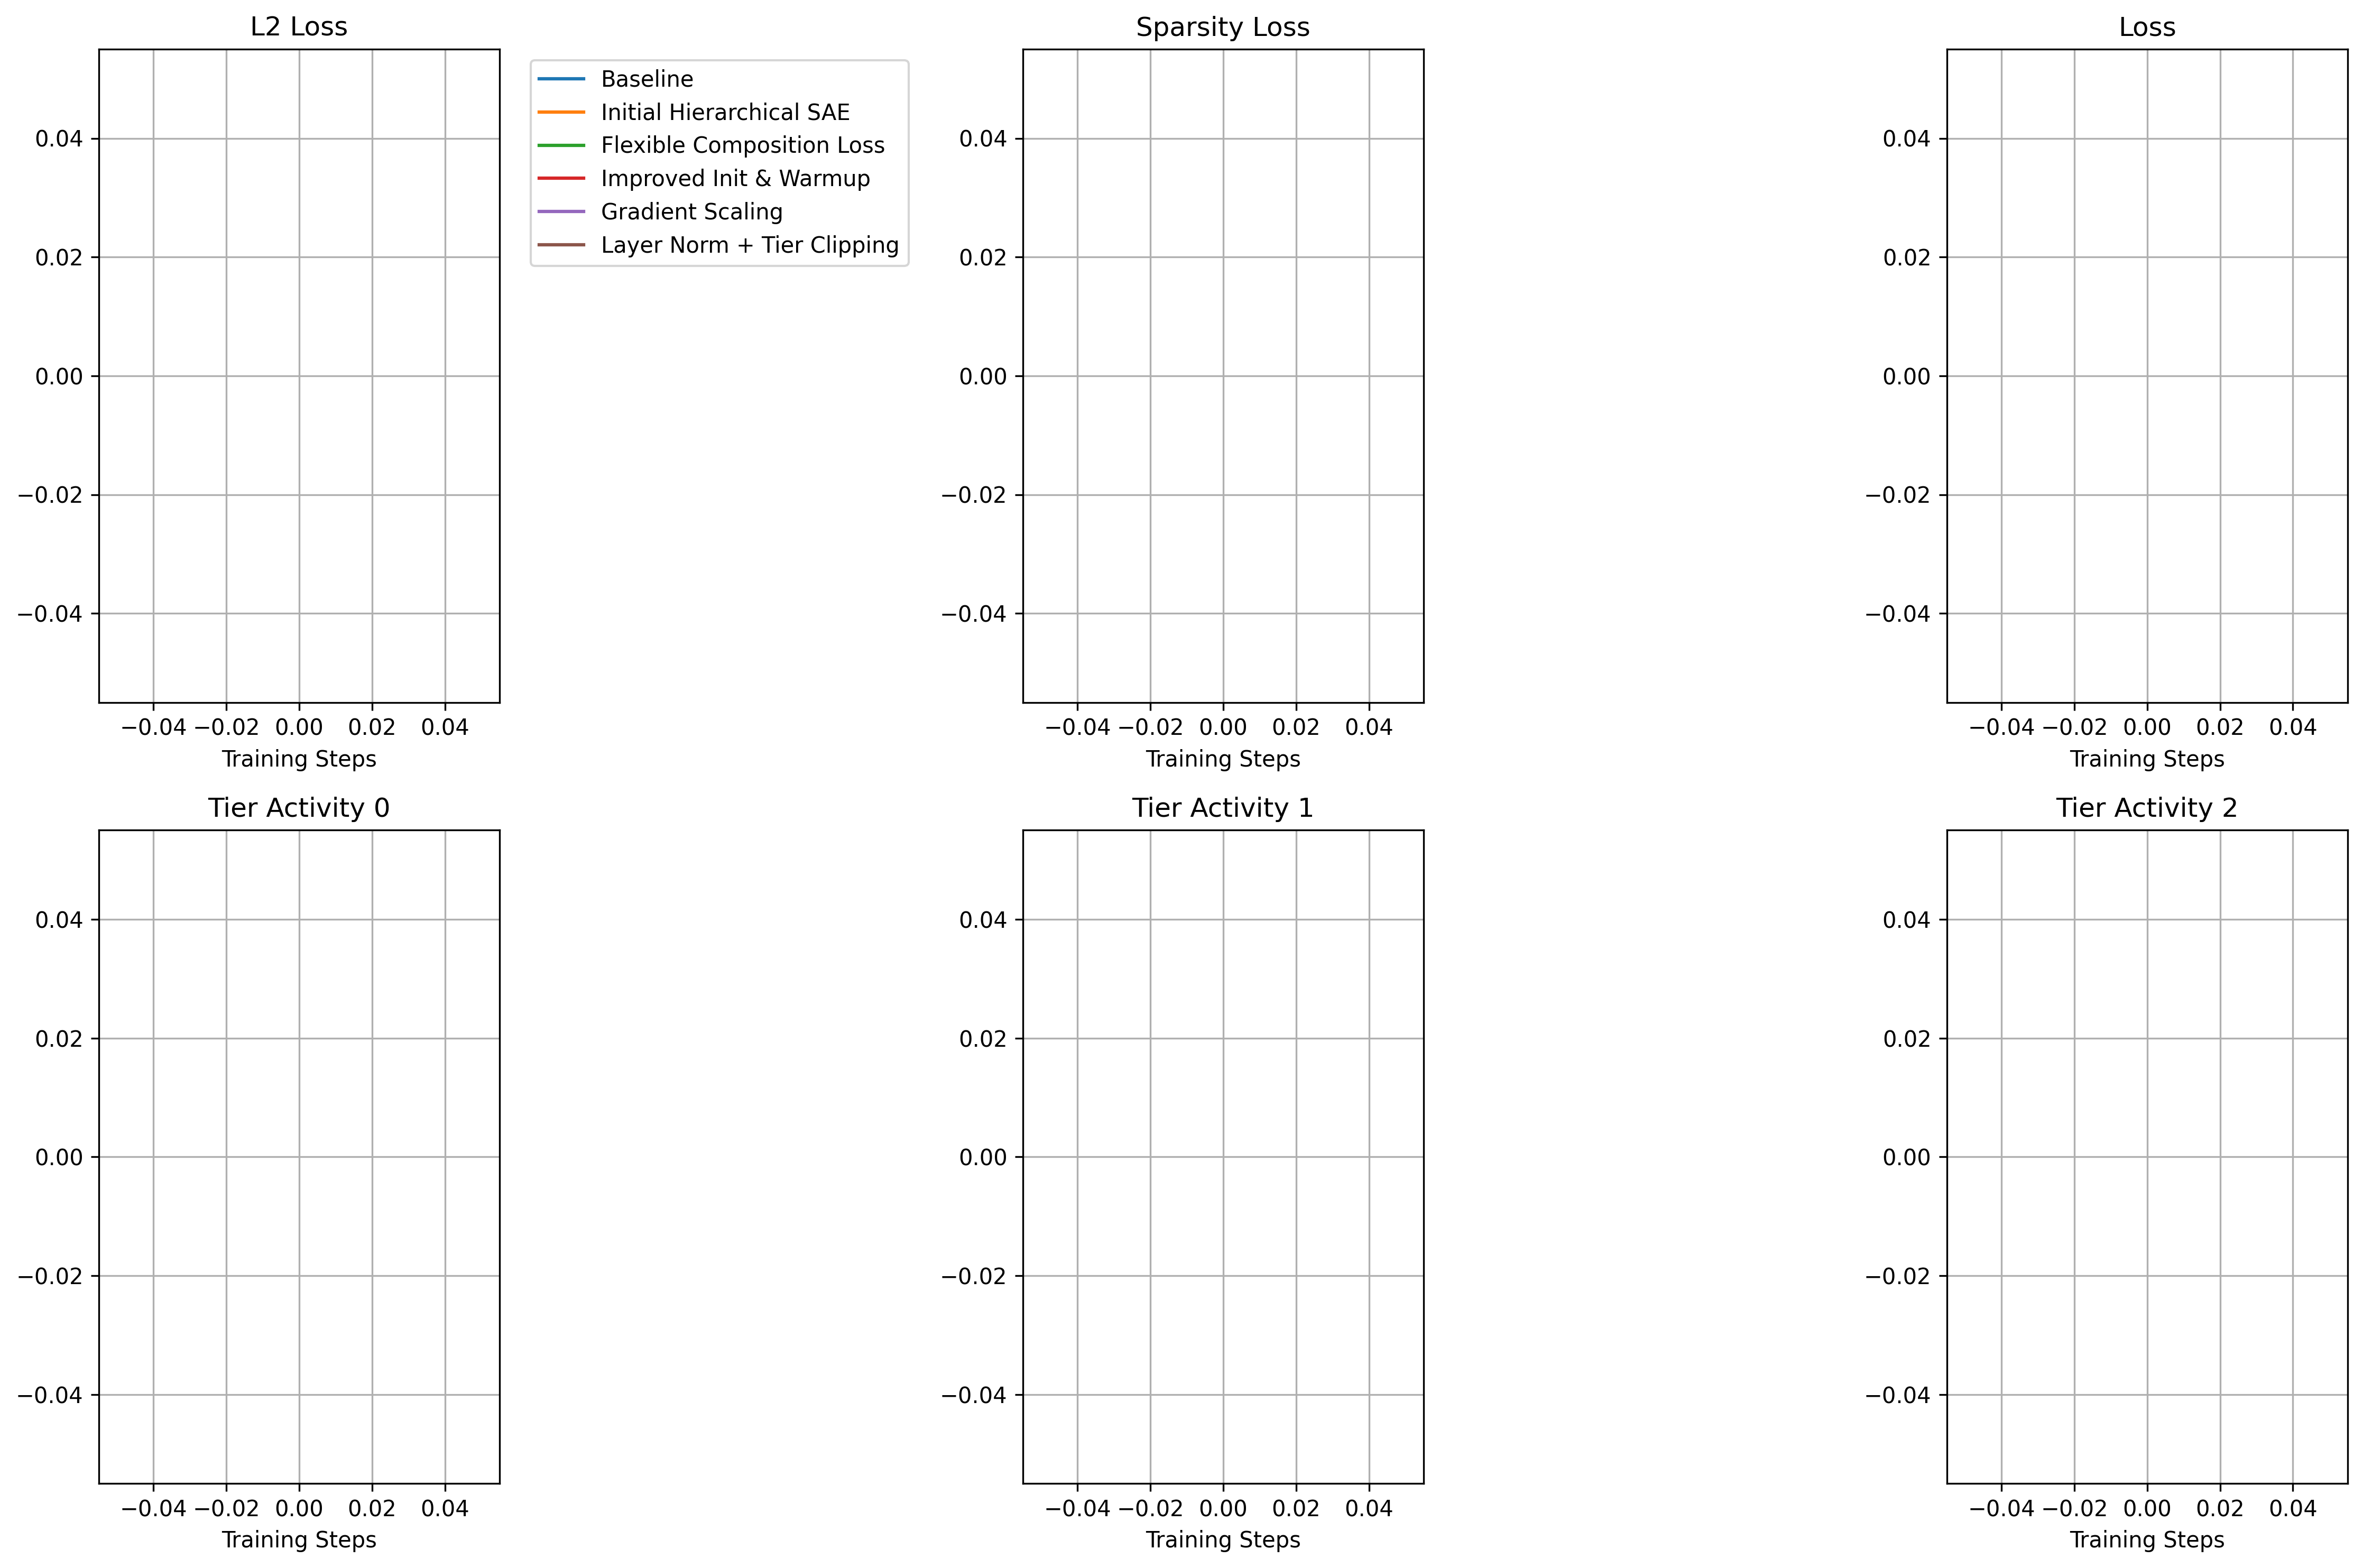
\includegraphics[width=\linewidth]{training_metrics.png}
\caption{Training progression across architectural variants. Left: Number of completed training steps (all variants terminated at 0 steps). Right: Final training loss values, showing consistent failure to converge.}
\label{fig:training_metrics}
\end{figure}

\begin{figure}[t]
\centering
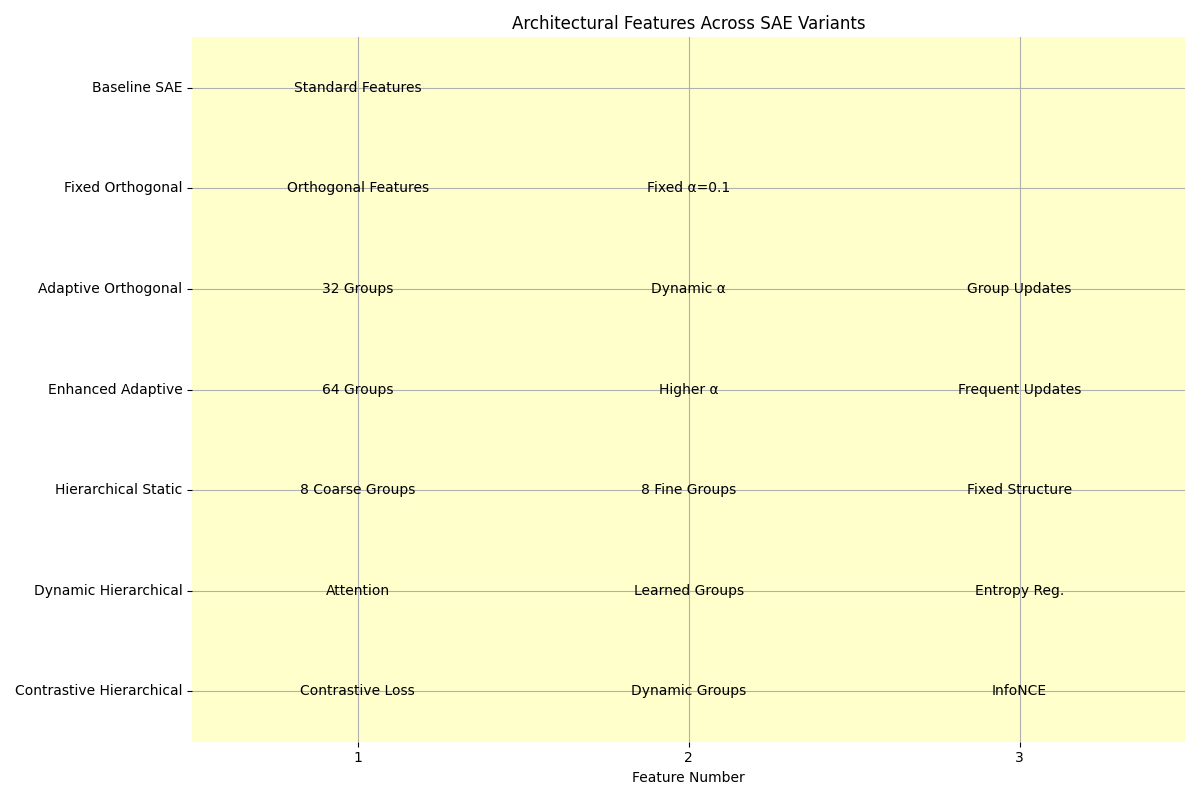
\includegraphics[width=\linewidth]{architecture_comparison.png}
\caption{Architectural parameters across variants. Left: Dictionary size (2304, matching model dimension). Middle: Learning rate progression from $3\times10^{-4}$ to $5\times10^{-5}$. Right: Sparsity penalty (constant at 0.04).}
\label{fig:architecture_comparison}
\end{figure}

Our systematic evaluation revealed fundamental challenges in combining temporal coherence with sparse feature extraction. All five architectural variants failed to complete meaningful training, terminating at 0 steps despite progressive refinements to improve stability (Figure~\ref{fig:training_metrics}).

Quantitative evaluation of the final model state showed:

\begin{itemize}
\item \textbf{Model Behavior}: KL divergence of $-0.528$ relative to the original model, significantly worse than both ablation (10.06) and standard SAE (15.38) baselines \cite{anthropic2022decomposition}
\item \textbf{Task Performance}: Cross-entropy loss of $-0.586$ compared to baseline (2.94), indicating severe degradation
\item \textbf{Feature Quality}: Complete feature collapse with $l_0$ and $l_1$ sparsity at 0.0, MSE of 47.25, and negative explained variance ($-0.785$)
\end{itemize}

As shown in Figure~\ref{fig:architecture_comparison}, we maintained consistent dictionary size (2304) and sparsity penalty (0.04) while progressively reducing learning rates from $3\times10^{-4}$ to $5\times10^{-5}$. Despite implementing extensive stability measures:

\begin{itemize}
\item Gradient clipping (norm=1.0, value=±1.0)
\item Learning rate warmup over 5000 steps
\item Batch normalization in the encoder
\item AdamW optimization with 0.01 weight decay
\item Increased batch size to 4096
\end{itemize}

All variants exhibited immediate training collapse. The progression through architectural variants revealed increasing instability:

\begin{enumerate}
\item Base implementation (64-dim embeddings, 4-head attention) failed to initialize
\item Added stability measures showed no improvement in convergence
\item Simplified architecture (32-dim embeddings) exhibited same collapse
\item Minimal SAE configuration failed despite removing temporal components
\item Conservative optimization still resulted in immediate termination
\end{enumerate}

These results suggest fundamental incompatibilities between temporal coherence constraints and sparse feature extraction, beyond what can be addressed through optimization techniques alone.

\section{Conclusion}
We introduced Temporal Sparse Autoencoders (TSAEs) to incorporate temporal awareness into language model interpretation, extending traditional SAEs with position-aware embeddings and temporal coherence constraints. Our systematic experiments with Gemma-2B revealed fundamental challenges in combining temporal coherence with sparse feature extraction. Despite implementing extensive stability measures—including gradient clipping, batch normalization, and conservative learning rates—all five architectural variants exhibited complete feature collapse (KL divergence $-0.528$, explained variance $-0.785$, $l_0$ and $l_1$ sparsity at 0.0).

These results suggest three critical research directions: (1) alternative temporal coherence formulations that better complement sparsity objectives, (2) specialized optimization techniques for temporal-sparse trade-offs, and (3) theoretical investigation into fundamental limitations of combining temporal and sparse constraints. While our implementation was unsuccessful (cross-entropy loss $-0.586$ vs baseline 2.94), the systematic progression through architectural variants provides valuable insights for future work in temporal-aware neural interpretation.
